\begin{pastexam}[label={px:ust-115-ee-ds-17}]{臺聯大電機類 115 學年度 第 17 題}
（單選；2 分）

If the pre-order of a binary tree is AB D E C F and the in-order is D B E A F C, what is its
post-order?

(A)~D E B F C A \qquad (B)~D E B C F A \qquad (C)~E D B F C A \qquad (D)~Not Unique
\end{pastexam}

\begin{pastsoln}
答案是 (A)。

用前序找根、中序分左右（資結書第~7.4~節，虛擬碼~7.5）：
\begin{enumerate}
\item 前序第一個 A 是根。 中序 D B E \textbar{} A \textbar{} F C：左子樹是 $\{D, B, E\}$，右子樹是
$\{F, C\}$。
\item 左子樹的前序是 B D E，根是 B；中序 D \textbar{} B \textbar{} E，D 是 B 的左孩子，E 是右孩子。
\item 右子樹的前序是 C F，根是 C；中序 F \textbar{} C，F 是 C 的左孩子。
\end{enumerate}
\begin{center}
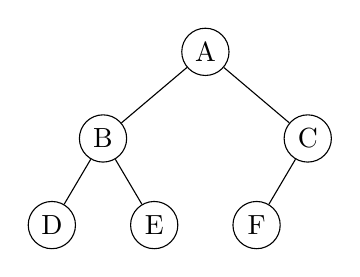
\begin{tikzpicture}[level distance=11mm, every node/.style={circle, draw, minimum size=6mm, inner sep=0pt},
  level 1/.style={sibling distance=26mm}, level 2/.style={sibling distance=13mm}]
\node {A}
  child {node {B} child {node {D}} child {node {E}}}
  child {node {C} child {node {F}} child[missing]};
\end{tikzpicture}
\end{center}
後序是「左、右、根」：左子樹 D E B，右子樹 F C，最後 A，得 D E B F C A。
驗證：這棵樹的前序是 A B D E C F、中序是 D B E A F C，和題目一致。

逐項檢查：
\begin{itemize}
\item (A) 對。
\item (B) D E B C F A：把 C、F 的順序弄反，等於把 F 當成 C 的父節點。 錯。
\item (C) E D B F C A：把 D、E 弄反，和中序 D B E（D 在 B 左邊）矛盾。 錯。
\item (D) 鍵值互不相同時，前序加中序唯一決定一棵二元樹（資結書定理~7.4），後序也唯一。 錯。
\end{itemize}
\end{pastsoln}
